\chapter{Comparing Venture and OpenBUGS}

In this chapter I perform an empirical comparison of the Venture and OpenBUGS probabilistic programming languages on several models, in order to gain a better understanding of these systems' strengths and limitations.

\section{Motivation}

A lot of current research in probabilistic programming is focused on achieving more efficient automatic inference on different types of models. This problem has been approached from many angles, ranging from the development of specialized inference methods that work well on certain, restricted, classes of models, to employing general inference techniques on models transformed by the application of optimization techniques similar to those used in compiler architecture. These distinct approaches have lead to the development of probabilistic programming languages (and implementations of these languages) which differ in significant ways.  At the moment, the relative benefits and drawbacks of these languages on different classes of models are not very well understood. 

In this chapter I attempt to take a step towards better understanding the relative benefits and drawbacks these languages by looking at two PPLs which fall at different ends of the specialization/generality spectrum. I do this by implementing a few different models and evaluating the performance of the two different PPL's inference engines on these models. The insight thus gained will give us an idea of where the current systems most need improving and thus reveal where future work should focus in order to alleviate these problems.

\section{Preliminaries}
\todo{Add background info on Venture and OpenBUGS}

\subsection{Webchurch's performance}
One alternative to Venture which I considered is WebChurch. WebChurch is a compiler which translated the Church PPL into JavaScript, and thus allows for in-browser execution.

I implemented a few very simple models (similar to the ones discussed below) in WebChurch, however the execution tended to hang even when conditioning on very few variables (less than 5) and when extracting very few samples (less than 100). Asking one of the WebChurch creators confirmed that the publicly available implementation is meant for didactic purposes and not designed to scale well. I therefore chose to focus only on Venture and OpenBUGS.

\subsection{Number of MCMC steps}
Venture and OpenBUGS have a different interpretation of what an MCMC step is. This difference must be taken into account so that the empirical results of the two PPLs are comparable.

Specifically, OpenBUGS updates all currently unconditioned variables during one step, whereas Venture only updates one, randomly chosen, variable. In order to correct for this, Venture will need to perform roughly (no. of OpenBUGS steps) * (no. of unconditioned variables) steps. Ideally, if we want both the amount of work and the number of samples generated by each PPL to be comparable, then we can specify the work that must be done by each PPL as:

\begin{table}[H]
  \centering
  \begin{tabular}{lll}
    \toprule
    & OpenBUGS & Venture \\
    \midrule
    Burned samples & B & V * B \\
    Extracted samples & S & S \\
    Inter-sample lag & L & V * L \\
    Total MCMC steps & B + L * S & V * (B + L * S) \\
    \bottomrule
  \end{tabular}
  \caption{Strategies for extracting S samples from a model with V unconditioned variables}
  \label{tab:noSteps}
\end{table}

However, in some cases it can make sense to not follow the above specification. For instance, when the performance gap between the two PPLs is very large, we may prefer not to generate very few samples with the faster PPL just so that the slower one can terminate the same amount of work in a reasonable timeframe. 

\section{Empirical results}
In this section consider a few simple models taken from the OpenBUGS model repository, and test inference performance on then for both OpenBUGS and Venture. \todo{Maybe also evaluate one model that's not from the OpenBUGS repository, since BUGS might be unreasonably optimized on its own models.}

\subsection{Tdf model description}
The Tdf models attempt to infer a Student t distribution's degrees of freedom, by considering 1,000 samples drawn from said Student t distribution. The Tdf models come in 3 variations, which just change the prior distrobution of the degrees of freedom parameter (called d). In the course discrete version d is drawn from the uniform discrete distribution between 2 and 50. In the fine discrete distribution, d is drawn uniformly from the set: \{2.0, 2.1, 2.2, \ldots 6.0\}. Finally, in the continuous version d is drawn from the continuous uniform distribution between 2 and 100. The models' OpenBUGS implementations and results can be found in the OpenBUGS model repository at: \url{http://www.openbugs.net/Examples/t-df.html}
\todo{add model pseudocode}

For all 3 Tdf models, OpenBUGS uses 1,000 steps for burn-in and then extracts 10,000 consecutive samples (i.e. using a lag of 1). The Tdf model has only 1 unconditioned variable and so, as explained in Table \ref{tab:noSteps}, this would correspond to \( 1 * (1000 + 1 * 10000) = 11,000 \) MCMC steps in Venture. However, as seen below, the different inference engines employed means that Venture needs more samples than OpenBUGS to derive a reasonable posterior estimate on this model. For this reason, I used a burn-in of 1000 and then extracted an additional 1000 samples using a lag of 100. The total number of steps performed by Venture is therefore \( 1000 + 1000 * 100 = 101,000 \).

\subsection{Tdf model true posteriors}
Given the simplicity of the Tdf models, we can calculate the true posteriors analytically.

\missingfigure{Add formula used to derive posterior, as in the log}

Using this formulation we calculate the true posteriors for all 3 Tdf model and get

\begin{figure}[H]
    \centering
    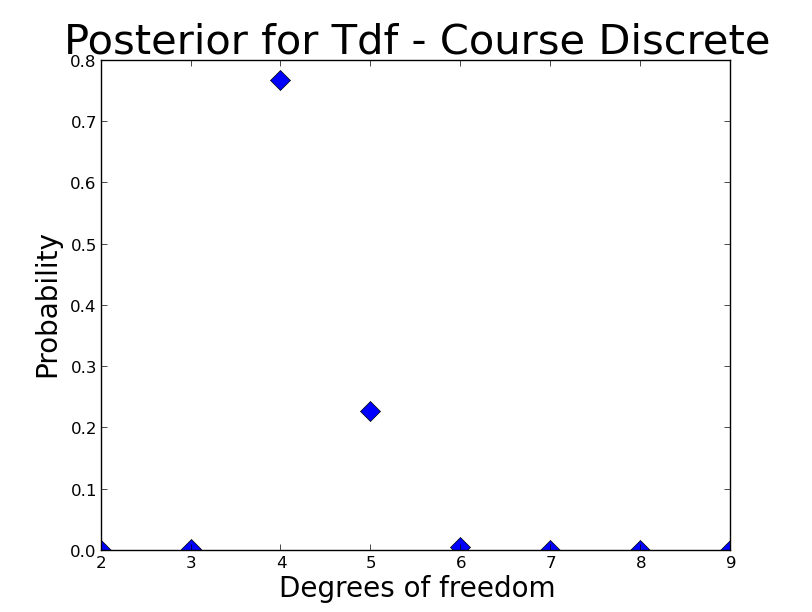
\includegraphics[width=\textwidth]{TdfCourseDiscPost.png}
    \caption{True posterior distribution for Tdf Course Discrete model.}
    \label{fig:tdfCourseDiscSamp}
\end{figure}

\begin{figure}[H]
    \centering
    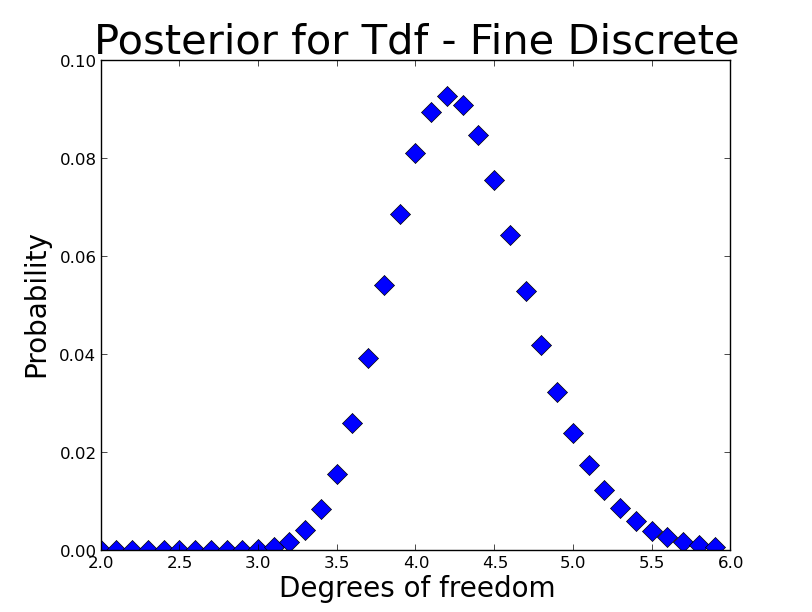
\includegraphics[width=\textwidth]{TdfFineDiscPost.png}
    \caption{True posterior distribution for Tdf Fine Discrete model.}
    \label{fig:tdfCourseDiscSamp}
\end{figure}

\begin{figure}[H]
    \centering
    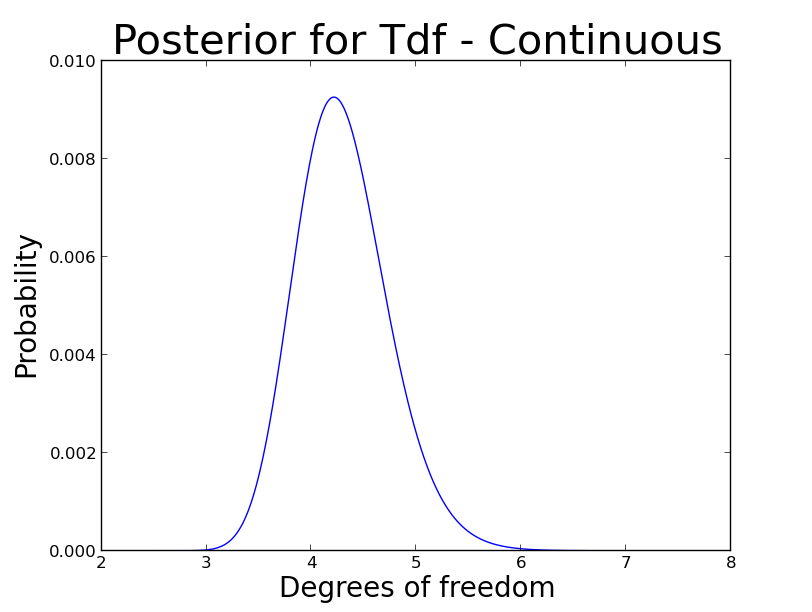
\includegraphics[width=\textwidth]{TdfContPost.png}
    \caption{True posterior distribution for Tdf Continuous model.}
    \label{fig:tdfCourseDiscSamp}
\end{figure}

\subsection{Tdf model results}
\todo{Add KL and KS difference results for these distributions}
\begin{figure}[H]
    \centering
    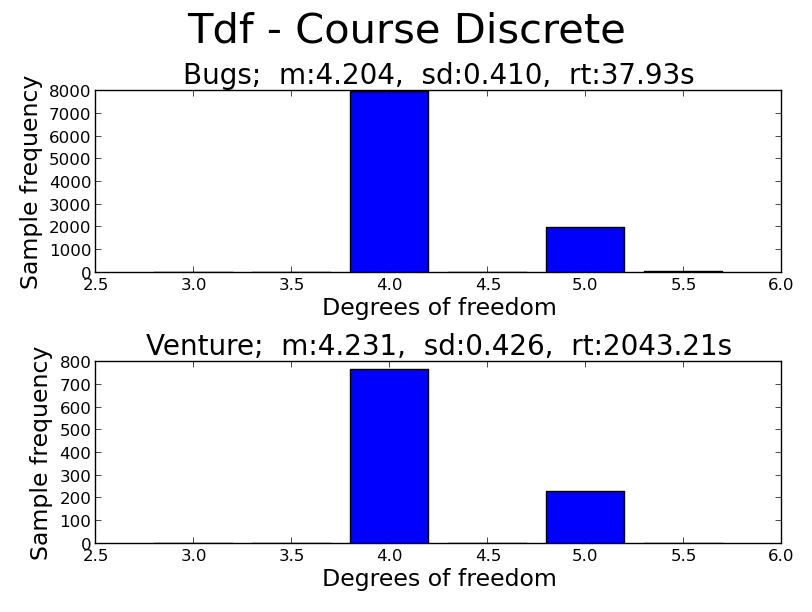
\includegraphics[width=\textwidth]{TdfCourseDiscSamps.png}
    \caption{Distributions obtained by the two PPLs on the course discrete model.}
    \label{fig:tdfCourseDiscSamp}
\end{figure}

On the course discrete model we see that the two PPLs obtain similar results but with a large gap in runtime. Venture runs $\sim$54 time more slowly than OpenBUGS. To get a better idea of the relative performance of the languages we can look at their speed of convergence to the true posterior.

\begin{figure}[H]
    \centering
    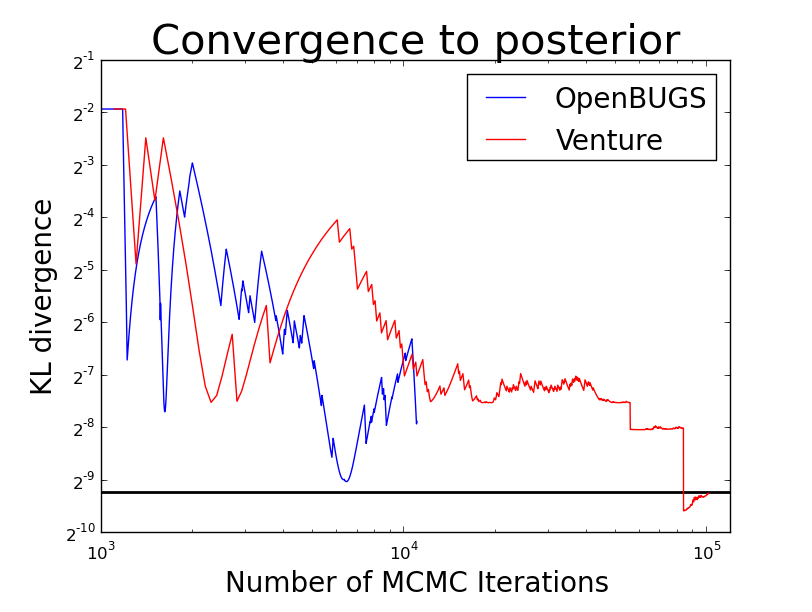
\includegraphics[width=\textwidth]{TdfCourseDiscConv.png}
    \caption{Rate of convergence of the two engines as the number of samples increases (first 1,000 samples are discarded as burn-in). The black line shows the KL divergence achieved by Venture after 101,000 inference steps.}
    \label{fig:tdfCourseDiscConv}
\end{figure}

Due to the course discrete prior, the convergence rate here is quite choppy and no significant conclusions can be drawn from this single run. 
\todo{Maybe do more runs and plot quartiles}

\begin{figure}[H]
    \centering
    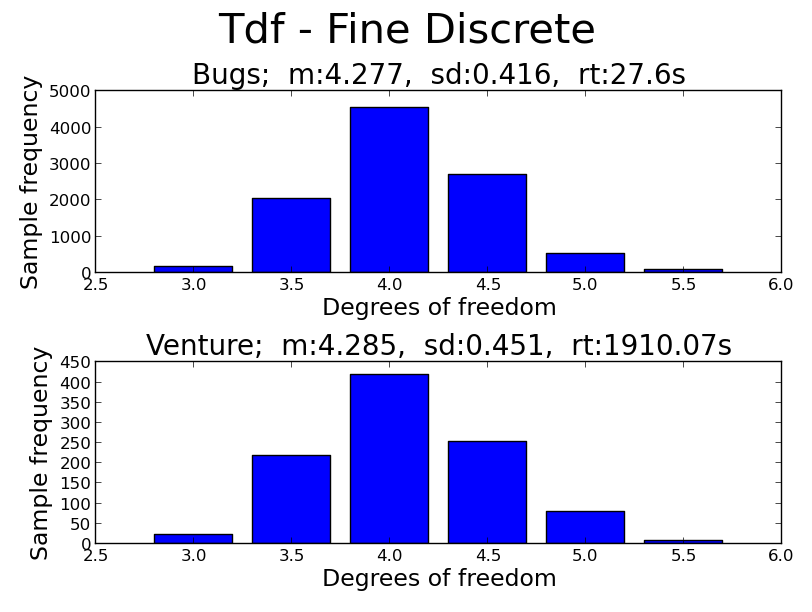
\includegraphics[width=\textwidth]{TdfFineDiscSamps.png}
    \caption{Distributions obtained by the two PPLs on the fine discrete model.}
    \label{fig:tdfFineDiscSamp}
\end{figure}

As with the course discrete case, the two engines obtain similar looking distributions, but the runtime gap actually worsens. Specifically, Venture now has a runtime $\sim$69 times larger than OpenBUGS.

Looking again at the convergence rate shows that Venture also does a worse job of inferring the true posterior, despite the longer runtime.

\begin{figure}[H]
    \centering
    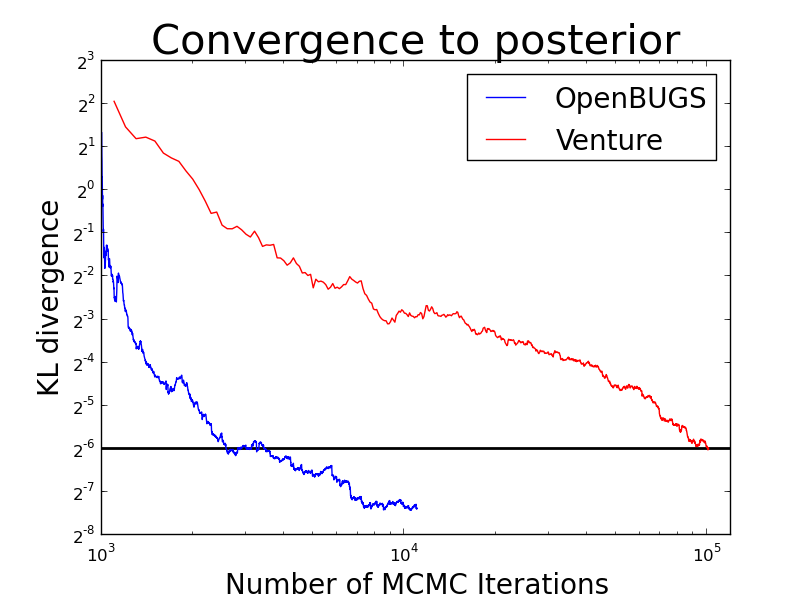
\includegraphics[width=\textwidth]{TdfFineDiscConv.png}
    \caption{Rate of convergence of the two engines as the number of samples increases (first 1,000 samples are discarded as burn-in). The black line shows the KL divergence achieved by Venture after 101,000 inference steps.}
    \label{fig:tdfFineDiscConv}
\end{figure}

The finer prior used here results in a much smoother convergence rate and so we can see that the KL divergence reached by Venture after 101,000 samples is achieved by OpenBUGS after only 3,000 (including the burn-in). Performing 3,000 MCMC steps in OpenBUGS takes 8.7 seconds, while Venture's run took 1910. So we may say that, reported to convergence to true posterior, Venture is $1910/8.7 = \sim 220$ times slower than OpenBUGS.

\begin{figure}[H]
    \centering
    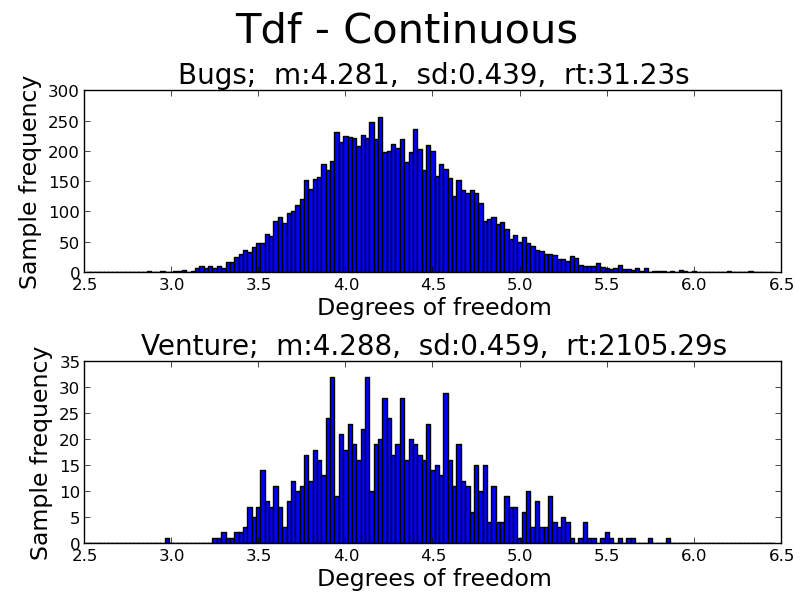
\includegraphics[width=\textwidth]{TdfContSamps.png}
    \caption{Distributions obtained by the two PPLs on the continuous model.}
    \label{fig:tdfContSamp}
\end{figure}

On the continuous case, not only does the runtime gap persist (Venture is again $\sim$68 times slower than OpenBUGS), but the distribution generated by Venture is also visibly noisier. One explanation for the noise could be the fact that, even though Venture is performing more MCMC iterations, due to the lag of 100 between extracted samples, it is actually generating only 1,000 samples compared to OpenBUGS' 10,000. 

To get a better idea of the PPL's performance we can once more look at their convergence rates.

\begin{figure}[H]
    \centering
    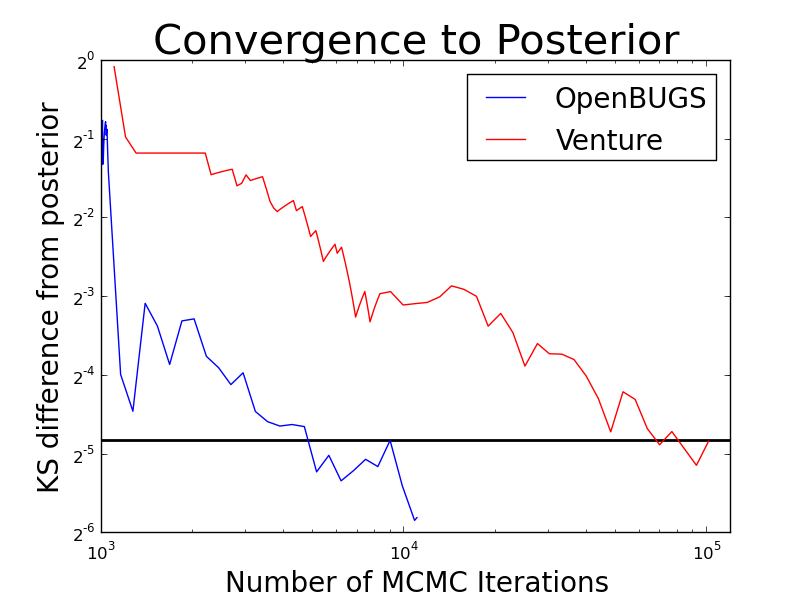
\includegraphics[width=\textwidth]{TdfContConv.png}
    \caption{Rate of convergence of the two engines as the number of samples increases (first 1,000 samples are discarded as burn-in). The black line shows the KS difference achieved by Venture after 101,000 inference steps.}
    \label{fig:tdfFineDiscConv}
\end{figure}

As with the fine discrete model, there seems to be a large qualitative gap between the performance of the two engines on this model. Thus the KS difference achieved by Venture after 101,000 MCMC iterations is reached by OpenBUGS after only 5,000. Additionally, while Venture takes 2105 seconds to reach this performance level, OpenBUGS does it in 16.5. Venture is therefore $2105/16.5 = \sim 127$ times slower than OpenBUGS on this model.

Based on these results we can say that Venture performs significantly worse then OpenBUGS on the Tdf model variants (with the last two variants exhibiting a slow-down of at least 2 orders of magnitude).

\section{Analysis of Venture's performance}

In order to understand why Venture seems to perform so badly on the Tdf models, we look at the distribution of runs of identical samples generated by the two engines.

\begin{figure}[H]
    \centering
    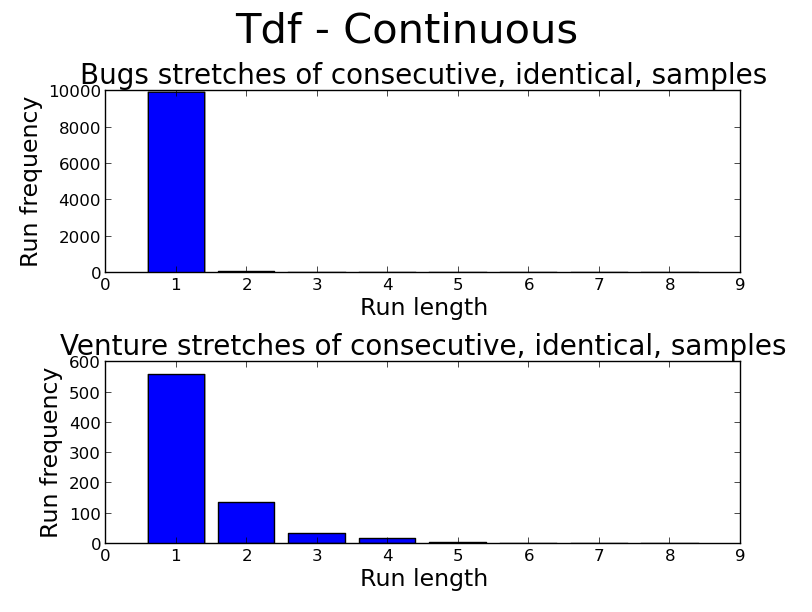
\includegraphics[width=\textwidth]{TdfContRuns.png}
    \caption{Number and size of identical sample runs generated by the two PPLs on the continuous model.}
    \label{fig:tdfContRun}
\end{figure}

Figure \ref{fig:tdfContRun} shows that Venture has a much higher propensity for identical sample runs than OpenBUGS. Keeping in mind that Venture takes a lag of 100 samples between each 2 extracted samples, we see that Venture exhibits several runs of over 500 MCMC iterations where the observed variable does not change at all. On the other hand, OpenBUGS has no two identical consecutive samples.

This difference can be explained by the different inference strategies employed by the two engines. Venture makes use of single-site Metropolis whereas OpenBUGS uses a slice sampler on one dimensional models such as Tdf \todo{saw this mentioned in a paper, need to find direct source or remove}. We take a closer look at these different inference techniques and their performance in Chapter \ref{whoKnows}.

\todo{Decide is there's anything worth reporting from the performance tests done on Venture. Log dates: 2014.02.19 and 2014.02.20}
